\chapter{IQ Representation}
\label{ch:iq-representation}

\begin{nontechnical}
\textbf{IQ representation is like describing a location on a map using X and Y coordinates}---it lets you pinpoint any radio signal position in 2D space!

\textbf{The clock analogy:}
\begin{itemize}
\item 12 o'clock position = I = max, Q = 0
\item 3 o'clock position = I = 0, Q = max
\item 6 o'clock position = I = -max, Q = 0
\item 9 o'clock position = I = 0, Q = -max
\item Any angle = unique IQ coordinate!
\end{itemize}

\textbf{Why two dimensions?} Radio waves have both \textbf{amplitude} (strength) and \textbf{phase} (timing). Two dimensions let you control BOTH simultaneously, doubling your data capacity compared to just varying amplitude.

\textbf{The magic trick:} One wire carries the I signal, another carries the Q signal. At the transmitter, they're combined using $90^\circ$ phase-shifted carriers. At the receiver, they're split apart the same way. Result: Two independent data channels on the same frequency!

\textbf{Real use:} Every smartphone, WiFi chip, and Software Defined Radio (SDR) processes IQ data internally. It's the universal language of digital communications.
\end{nontechnical}

\section{Overview}

\textbf{IQ Representation} (also called \textbf{complex baseband representation} or \textbf{quadrature representation}) is the fundamental mathematical framework for describing and processing modulated signals in modern communications systems.

\begin{keyconcept}
IQ representation provides a \textbf{unified framework} for analyzing all linear modulation schemes (BPSK, QPSK, QAM, etc.) using complex arithmetic. This eliminates the need for separate carrier frequency analysis and simplifies both mathematical derivations and DSP implementations.
\end{keyconcept}

Any bandpass signal can be decomposed into two orthogonal baseband components:
\begin{itemize}
\item \textbf{I (In-phase):} The component aligned with the carrier wave $\cos(2\pi f_c t)$
\item \textbf{Q (Quadrature):} The component aligned with the $90^\circ$ phase-shifted carrier $\sin(2\pi f_c t)$
\end{itemize}

This decomposition is fundamental to:
\begin{enumerate}
\item \textbf{Digital signal processing:} All modern transceivers operate on IQ samples
\item \textbf{Constellation diagrams:} Visual representation of modulation schemes
\item \textbf{Channel equalization:} Correcting distortion in I and Q independently
\item \textbf{Carrier recovery:} Estimating and correcting phase/frequency offsets
\end{enumerate}

\section{Mathematical Description}

\subsection{Passband Signal Representation}

A general bandpass signal can be expressed as:
\begin{equation}
s(t) = A(t) \cos[2\pi f_c t + \phi(t)]
\end{equation}
where:
\begin{itemize}
\item $A(t)$ = time-varying amplitude envelope
\item $f_c$ = carrier frequency (Hz)
\item $\phi(t)$ = time-varying phase
\end{itemize}

Using the trigonometric identity $\cos(\alpha + \beta) = \cos\alpha\cos\beta - \sin\alpha\sin\beta$:
\begin{equation}
s(t) = A(t)\cos[\phi(t)] \cos(2\pi f_c t) - A(t)\sin[\phi(t)] \sin(2\pi f_c t)
\end{equation}

\subsection{IQ Component Definition}

Define the baseband IQ components:
\begin{equation}
I(t) = A(t)\cos[\phi(t)]
\end{equation}
\begin{equation}
Q(t) = A(t)\sin[\phi(t)]
\end{equation}

Then the passband signal becomes:
\begin{equation}
s(t) = I(t) \cos(2\pi f_c t) - Q(t) \sin(2\pi f_c t)
\end{equation}
where:
\begin{itemize}
\item $I(t)$ = in-phase component (real part)
\item $Q(t)$ = quadrature component (imaginary part)
\item The minus sign is a convention from the analytic signal representation
\end{itemize}

\begin{calloutbox}{Physical Interpretation}
The I component modulates a cosine carrier (reference phase), while the Q component modulates a sine carrier ($90^\circ$ phase shift). These two carriers are \textbf{orthogonal}---they don't interfere with each other, allowing independent transmission of two data streams simultaneously.
\end{calloutbox}

\subsection{Complex Baseband Representation}

The IQ signal can be compactly written using complex notation:
\begin{equation}
s_{\mathrm{baseband}}(t) = I(t) + jQ(t)
\end{equation}
where $j = \sqrt{-1}$ is the imaginary unit.

The passband signal is then:
\begin{equation}
s(t) = \mathrm{Re}\{s_{\mathrm{baseband}}(t) \cdot e^{j2\pi f_c t}\}
\end{equation}

\textbf{Amplitude and phase recovery:}
\begin{equation}
A(t) = |s_{\mathrm{baseband}}(t)| = \sqrt{I^2(t) + Q^2(t)}
\end{equation}
\begin{equation}
\phi(t) = \arg[s_{\mathrm{baseband}}(t)] = \arctan\left(\frac{Q(t)}{I(t)}\right)
\end{equation}

\subsection{IQ Plane Visualization}

The IQ plane is a 2D coordinate system where any complex baseband signal is represented as a point:

\begin{center}
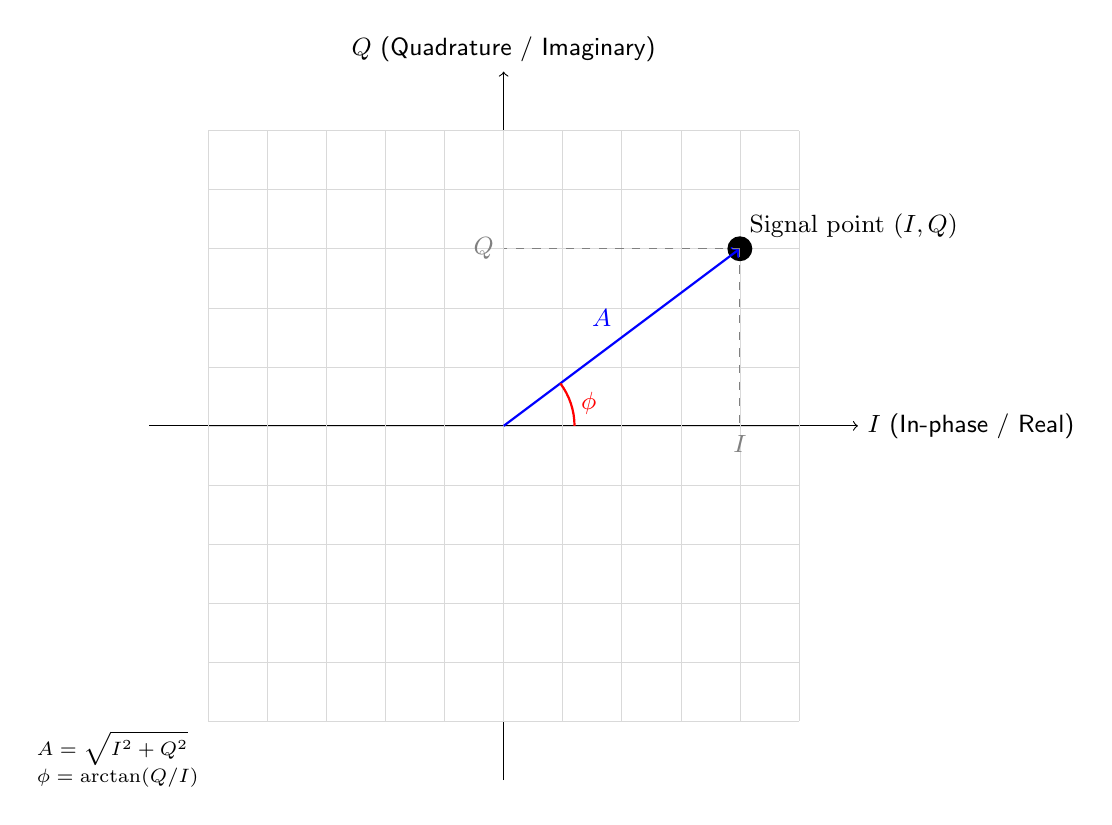
\begin{tikzpicture}[scale=1.5]
% Axes
\draw[->] (-3,0) -- (3,0) node[right] {\sffamily\small $I$ (In-phase / Real)};
\draw[->] (0,-3) -- (0,3) node[above] {\sffamily\small $Q$ (Quadrature / Imaginary)};

% Grid
\draw[very thin,gray!30] (-2.5,-2.5) grid[step=0.5] (2.5,2.5);

% Example signal point
\fill[black] (2,1.5) circle (3pt);
\draw[->,thick,blue] (0,0) -- (2,1.5) node[midway,above left,font=\small] {$A$};

% Projections
\draw[dashed,gray] (2,1.5) -- (2,0) node[below,font=\small] {$I$};
\draw[dashed,gray] (2,1.5) -- (0,1.5) node[left,font=\small] {$Q$};

% Phase angle
\draw[thick,red] (0.6,0) arc (0:36.87:0.6) node[midway,right,font=\small] {$\phi$};

% Labels
\node[above right,font=\small] at (2,1.5) {Signal point $(I,Q)$};
\node[below left,font=\scriptsize,align=left] at (-2.5,-2.5) {$A = \sqrt{I^2 + Q^2}$\\$\phi = \arctan(Q/I)$};
\end{tikzpicture}
\end{center}

Any signal point can be described equivalently by:
\begin{itemize}
\item \textbf{Cartesian:} $(I, Q)$ coordinates
\item \textbf{Polar:} Amplitude $A$ and phase $\phi$
\item \textbf{Complex:} $s = I + jQ = Ae^{j\phi}$
\end{itemize}

\section{Modulation and Demodulation}

\subsection{IQ Modulator (Transmitter)}

The IQ modulator converts baseband IQ samples into a passband RF signal:

\begin{center}
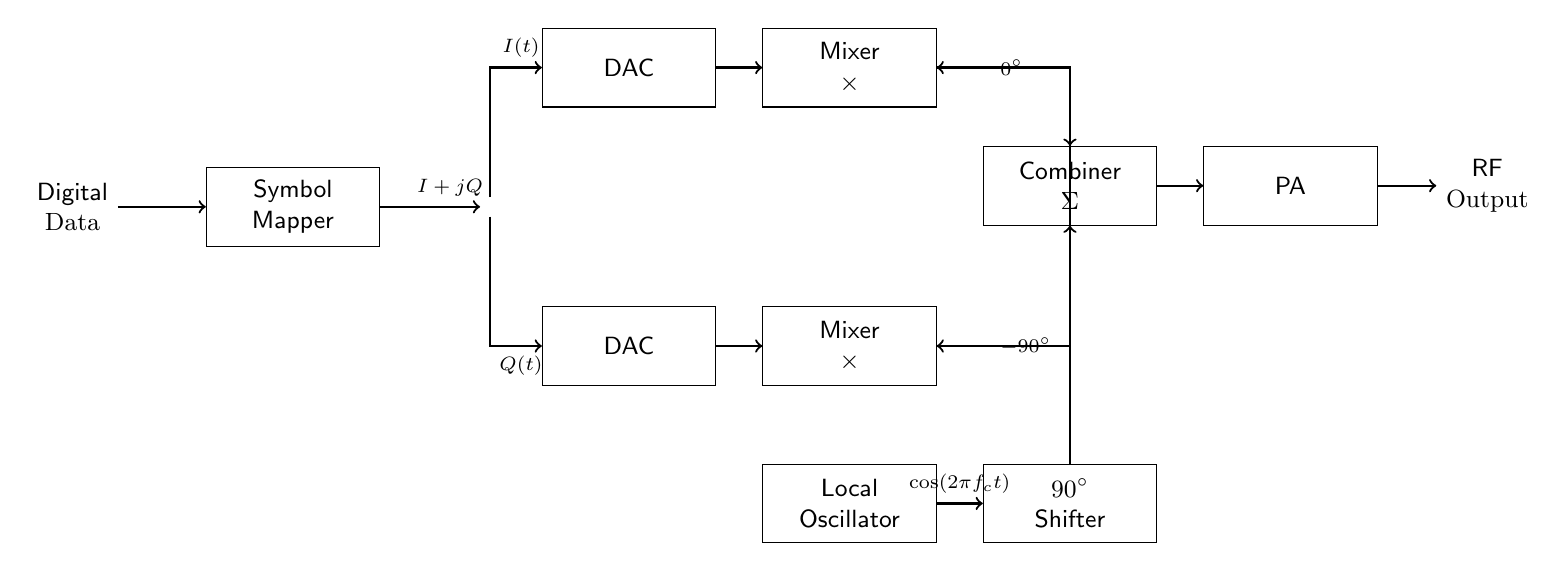
\begin{tikzpicture}[
  block/.style={rectangle, draw, minimum width=2.2cm, minimum height=1cm, font=\sffamily\small, align=center},
  node distance=2.2cm,
  font=\small
]
% Input
\node[align=center] (data) {\sffamily Digital\\Data};
\node[block, right of=data, node distance=2.8cm] (mapper) {Symbol\\Mapper};
\node[right of=mapper, node distance=2.5cm] (split) {};

% I path
\node[block, above right of=split, node distance=2.5cm] (dac_i) {DAC};
\node[block, right of=dac_i, node distance=2.8cm] (mult_i) {Mixer\\$\times$};

% Q path  
\node[block, below right of=split, node distance=2.5cm] (dac_q) {DAC};
\node[block, right of=dac_q, node distance=2.8cm] (mult_q) {Mixer\\$\times$};

% Local oscillator
\node[block, below of=mult_q, node distance=2cm] (lo) {Local\\Oscillator};
\node[block, right of=lo, node distance=2.8cm] (phase) {$90^\circ$\\Shifter};

% Combiner
\node[block, right of=mult_i, node distance=2.8cm, yshift=-1.5cm] (sum) {Combiner\\$\Sigma$};
\node[block, right of=sum, node distance=2.8cm] (amp) {PA};
\node[align=center, right of=amp, node distance=2.5cm] (output) {\sffamily RF\\Output};

% Connections
\draw[->,thick] (data) -- (mapper);
\draw[->,thick] (mapper) -- (split) node[above,pos=0.7,font=\scriptsize] {$I+jQ$};
\draw[->,thick] (split) |- (dac_i) node[above,pos=0.8,font=\scriptsize] {$I(t)$};
\draw[->,thick] (split) |- (dac_q) node[below,pos=0.8,font=\scriptsize] {$Q(t)$};
\draw[->,thick] (dac_i) -- (mult_i);
\draw[->,thick] (dac_q) -- (mult_q);
\draw[->,thick] (lo) -- (phase) node[above,midway,font=\scriptsize] {$\cos(2\pi f_c t)$};
\draw[->,thick] (phase) |- (mult_i) node[right,pos=0.8,font=\scriptsize] {$0^\circ$};
\draw[->,thick] (phase) |- (mult_q) node[right,pos=0.8,font=\scriptsize] {$-90^\circ$};
\draw[->,thick] (mult_i) -| (sum);
\draw[->,thick] (mult_q) -| (sum);
\draw[->,thick] (sum) -- (amp);
\draw[->,thick] (amp) -- (output);
\end{tikzpicture}
\end{center}

\textbf{Process:}
\begin{enumerate}
\item \textbf{Symbol mapping:} Convert bits to complex symbols $I + jQ$
\item \textbf{Digital-to-analog conversion:} Generate analog $I(t)$ and $Q(t)$ waveforms
\item \textbf{Upconversion:}
  \begin{itemize}
  \item I path: Multiply by $\cos(2\pi f_c t)$
  \item Q path: Multiply by $-\sin(2\pi f_c t)$ (using $90^\circ$ phase shift)
  \end{itemize}
\item \textbf{Combination:} Sum I and Q paths to create $s(t) = I(t)\cos(2\pi f_c t) - Q(t)\sin(2\pi f_c t)$
\item \textbf{Amplification:} Power amplifier boosts signal for transmission
\end{enumerate}

\subsection{IQ Demodulator (Receiver)}

The IQ demodulator extracts baseband IQ components from the received RF signal:

\begin{center}
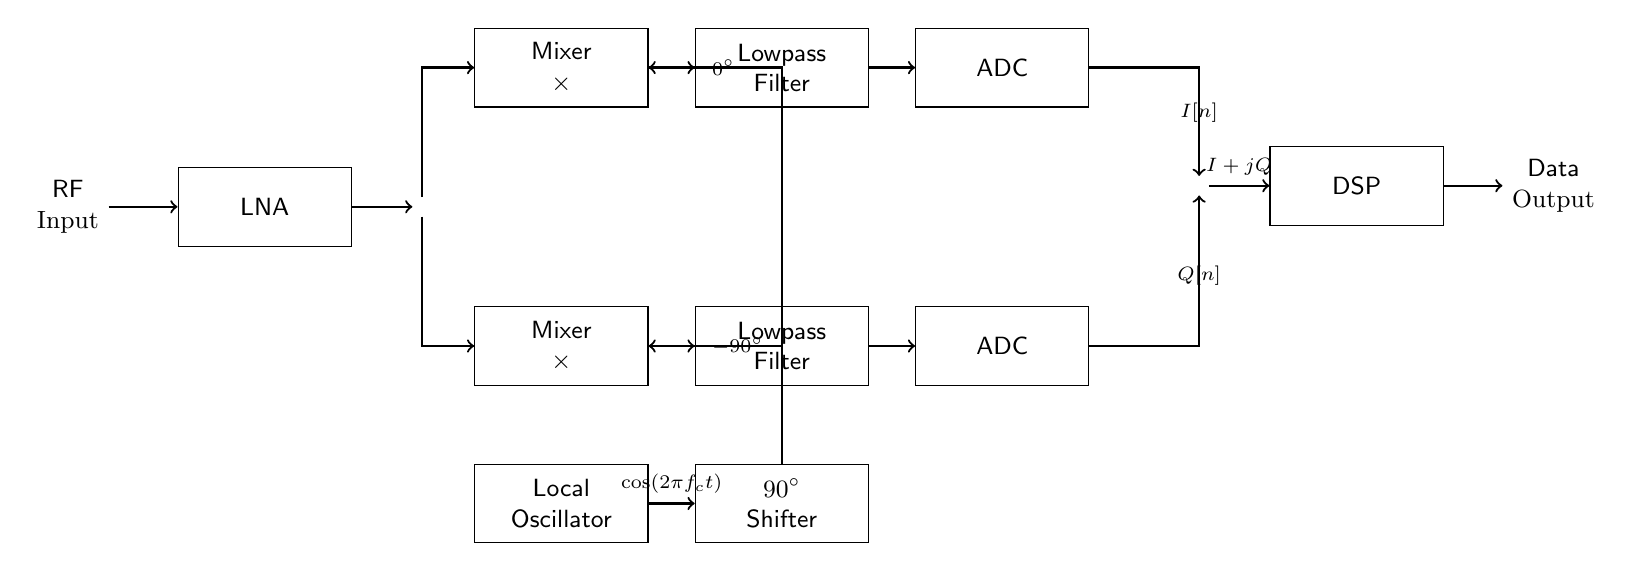
\begin{tikzpicture}[
  block/.style={rectangle, draw, minimum width=2.2cm, minimum height=1cm, font=\sffamily\small, align=center},
  node distance=2.2cm,
  font=\small
]
% Input
\node[align=center] (input) {\sffamily RF\\Input};
\node[block, right of=input, node distance=2.5cm] (lna) {LNA};
\node[right of=lna, node distance=2cm] (split) {};

% I path
\node[block, above right of=split, node distance=2.5cm] (mult_i) {Mixer\\$\times$};
\node[block, right of=mult_i, node distance=2.8cm] (lpf_i) {Lowpass\\Filter};
\node[block, right of=lpf_i, node distance=2.8cm] (adc_i) {ADC};

% Q path
\node[block, below right of=split, node distance=2.5cm] (mult_q) {Mixer\\$\times$};
\node[block, right of=mult_q, node distance=2.8cm] (lpf_q) {Lowpass\\Filter};
\node[block, right of=lpf_q, node distance=2.8cm] (adc_q) {ADC};

% Local oscillator
\node[block, below of=mult_q, node distance=2cm] (lo) {Local\\Oscillator};
\node[block, right of=lo, node distance=2.8cm] (phase) {$90^\circ$\\Shifter};

% Output
\node[right of=adc_i, node distance=2.5cm, yshift=-1.5cm] (combine) {};
\node[block, right of=combine, node distance=2cm] (dsp) {DSP};
\node[align=center, right of=dsp, node distance=2.5cm] (output) {\sffamily Data\\Output};

% Connections
\draw[->,thick] (input) -- (lna);
\draw[->,thick] (lna) -- (split);
\draw[->,thick] (split) |- (mult_i);
\draw[->,thick] (split) |- (mult_q);
\draw[->,thick] (mult_i) -- (lpf_i);
\draw[->,thick] (mult_q) -- (lpf_q);
\draw[->,thick] (lpf_i) -- (adc_i);
\draw[->,thick] (lpf_q) -- (adc_q);
\draw[->,thick] (lo) -- (phase) node[above,midway,font=\scriptsize] {$\cos(2\pi f_c t)$};
\draw[->,thick] (phase) |- (mult_i) node[right,pos=0.8,font=\scriptsize] {$0^\circ$};
\draw[->,thick] (phase) |- (mult_q) node[right,pos=0.8,font=\scriptsize] {$-90^\circ$};
\draw[->,thick] (adc_i) -| (combine) node[above,pos=0.8,font=\scriptsize] {$I[n]$};
\draw[->,thick] (adc_q) -| (combine) node[below,pos=0.8,font=\scriptsize] {$Q[n]$};
\draw[->,thick] (combine) -- (dsp) node[above,midway,font=\scriptsize] {$I+jQ$};
\draw[->,thick] (dsp) -- (output);
\end{tikzpicture}
\end{center}

\textbf{Process:}
\begin{enumerate}
\item \textbf{Amplification:} Low-noise amplifier (LNA) boosts weak RF signal
\item \textbf{Downconversion:}
  \begin{itemize}
  \item I path: Multiply by $\cos(2\pi f_c t)$ to extract $I(t)$
  \item Q path: Multiply by $-\sin(2\pi f_c t)$ to extract $Q(t)$
  \end{itemize}
\item \textbf{Lowpass filtering:} Remove high-frequency $2f_c$ components
\item \textbf{Analog-to-digital conversion:} Sample $I(t)$ and $Q(t)$ to get $I[n]$ and $Q[n]$
\item \textbf{Digital processing:} Demodulate symbols, equalize channel, decode data
\end{enumerate}

\begin{warningbox}
\textbf{Phase coherence is essential.} The local oscillator in the receiver must be frequency-locked AND phase-locked to the transmitter carrier. Even small phase errors $\phi_e$ reduce signal amplitude by $\cos(\phi_e)$ and cause IQ cross-talk. At $\phi_e = 90^\circ$, I and Q are completely swapped!
\end{warningbox}

\section{Constellation Diagrams}

A \textbf{constellation diagram} is a scatter plot of IQ samples, with I on the horizontal axis and Q on the vertical axis. Each point represents a transmitted symbol.

\subsection{QPSK Example}

QPSK uses 4 constellation points at $45^\circ$, $135^\circ$, $225^\circ$, and $315^\circ$:

\begin{center}
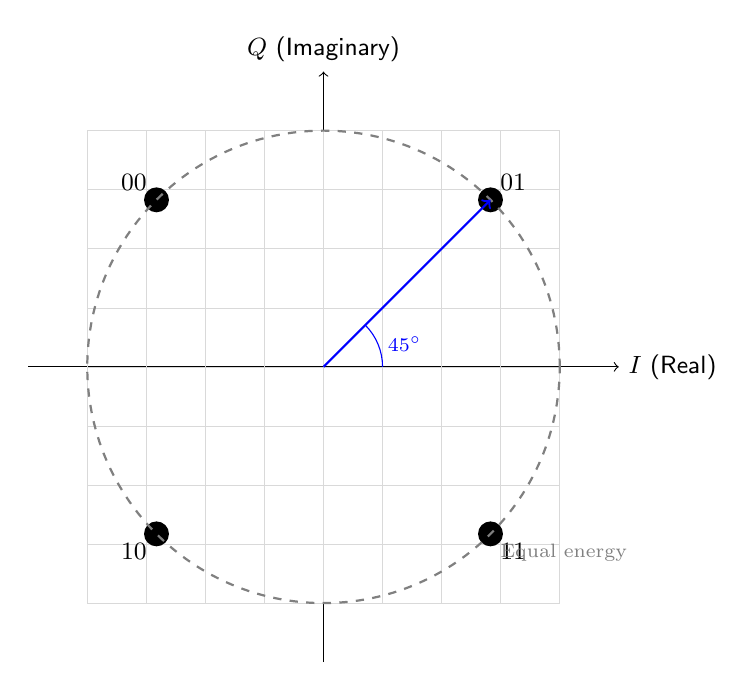
\begin{tikzpicture}[scale=1.5]
% Axes
\draw[->] (-2.5,0) -- (2.5,0) node[right] {\sffamily\small $I$ (Real)};
\draw[->] (0,-2.5) -- (0,2.5) node[above] {\sffamily\small $Q$ (Imaginary)};

% Grid
\draw[very thin,gray!30] (-2,-2) grid[step=0.5] (2,2);

% Constellation points
\fill[black] (1.414,1.414) circle (3pt);
\fill[black] (-1.414,1.414) circle (3pt);
\fill[black] (-1.414,-1.414) circle (3pt);
\fill[black] (1.414,-1.414) circle (3pt);

% Labels
\node[above right,font=\small] at (1.414,1.414) {01};
\node[above left,font=\small] at (-1.414,1.414) {00};
\node[below left,font=\small] at (-1.414,-1.414) {10};
\node[below right,font=\small] at (1.414,-1.414) {11};

% Energy circle
\draw[thick,gray,dashed] (0,0) circle (2);
\node[below right,gray,font=\scriptsize] at (1.414,-1.414) {Equal energy};

% Phase angles
\draw[->,blue,thick] (0,0) -- (1.414,1.414);
\draw[blue] (0.5,0) arc (0:45:0.5) node[midway,right,font=\scriptsize] {$45^\circ$};
\end{tikzpicture}
\end{center}

\textbf{QPSK symbol table:}

\begin{center}
\begin{tabular}{@{}ccccr@{}}
\toprule
Bits & $I$ & $Q$ & Complex & Phase \\
\midrule
00 & $-\frac{1}{\sqrt{2}}$ & $+\frac{1}{\sqrt{2}}$ & $-0.707+j0.707$ & $135^\circ$ \\
01 & $+\frac{1}{\sqrt{2}}$ & $+\frac{1}{\sqrt{2}}$ & $+0.707+j0.707$ & $45^\circ$ \\
10 & $-\frac{1}{\sqrt{2}}$ & $-\frac{1}{\sqrt{2}}$ & $-0.707-j0.707$ & $225^\circ$ \\
11 & $+\frac{1}{\sqrt{2}}$ & $-\frac{1}{\sqrt{2}}$ & $+0.707-j0.707$ & $315^\circ$ \\
\bottomrule
\end{tabular}
\end{center}

Note: Amplitudes are normalized so that $\sqrt{I^2 + Q^2} = 1$.

\subsection{Effect of AWGN Noise}

When Additive White Gaussian Noise (AWGN) is added, the received IQ samples become:
\begin{equation}
I_{\mathrm{rx}} = I_{\mathrm{tx}} + N_I
\end{equation}
\begin{equation}
Q_{\mathrm{rx}} = Q_{\mathrm{tx}} + N_Q
\end{equation}
where $N_I$ and $N_Q$ are independent Gaussian random variables with zero mean and variance $\sigma^2 = N_0/2$.

\begin{center}
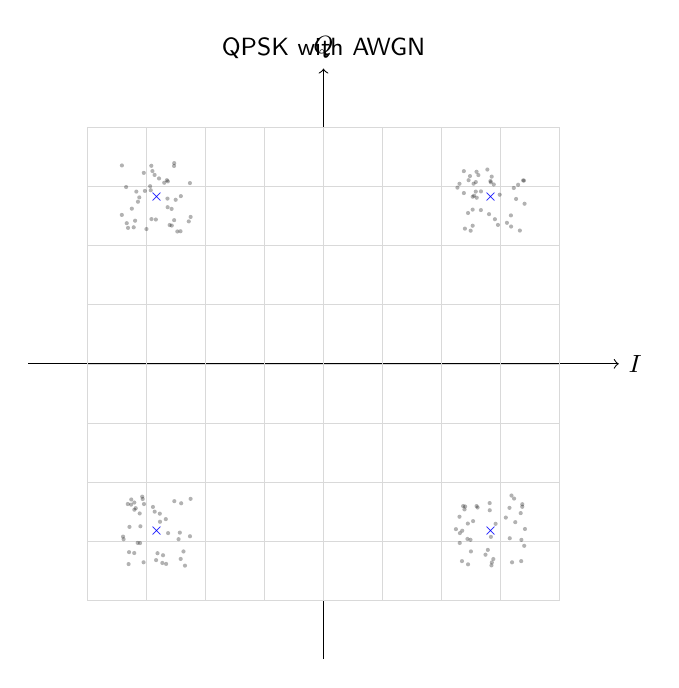
\begin{tikzpicture}[scale=1.5]
% Axes
\draw[->] (-2.5,0) -- (2.5,0) node[right] {\sffamily\small $I$};
\draw[->] (0,-2.5) -- (0,2.5) node[above] {\sffamily\small $Q$};

% Grid
\draw[very thin,gray!30] (-2,-2) grid[step=0.5] (2,2);

% Ideal constellation points (hidden under noise cloud)
\node[font=\tiny,blue] at (1.414,1.414) {$\times$};
\node[font=\tiny,blue] at (-1.414,1.414) {$\times$};
\node[font=\tiny,blue] at (-1.414,-1.414) {$\times$};
\node[font=\tiny,blue] at (1.414,-1.414) {$\times$};

% Noise clouds (simulated with random dots)
\foreach \i in {1,...,40} {
  \pgfmathsetmacro{\x}{1.414 + 0.3*rand}
  \pgfmathsetmacro{\y}{1.414 + 0.3*rand}
  \fill[black,opacity=0.3] (\x,\y) circle (0.5pt);
}
\foreach \i in {1,...,40} {
  \pgfmathsetmacro{\x}{-1.414 + 0.3*rand}
  \pgfmathsetmacro{\y}{1.414 + 0.3*rand}
  \fill[black,opacity=0.3] (\x,\y) circle (0.5pt);
}
\foreach \i in {1,...,40} {
  \pgfmathsetmacro{\x}{-1.414 + 0.3*rand}
  \pgfmathsetmacro{\y}{-1.414 + 0.3*rand}
  \fill[black,opacity=0.3] (\x,\y) circle (0.5pt);
}
\foreach \i in {1,...,40} {
  \pgfmathsetmacro{\x}{1.414 + 0.3*rand}
  \pgfmathsetmacro{\y}{-1.414 + 0.3*rand}
  \fill[black,opacity=0.3] (\x,\y) circle (0.5pt);
}

\node[above,font=\small\sffamily] at (0,2.5) {QPSK with AWGN};
\end{tikzpicture}
\end{center}

The received symbols form \textbf{clouds} instead of points. Decision boundaries are drawn halfway between constellation points. If noise pushes a received sample across the boundary, a \textbf{symbol error} occurs.

\begin{keyconcept}
The \textbf{Euclidean distance} between constellation points determines error probability. Larger separation = better noise immunity. This is why QPSK outperforms 16-QAM at low SNR, despite lower spectral efficiency.
\end{keyconcept}

\section{Mathematical Derivations}

\subsection{Orthogonality of I and Q Carriers}

The I and Q carriers are mathematically orthogonal over a symbol period $T$:
\begin{equation}
\int_0^T \cos(2\pi f_c t) \cdot \sin(2\pi f_c t) \, dt = 0
\end{equation}

This orthogonality ensures that I and Q components can be independently recovered at the receiver without cross-talk (assuming perfect synchronization).

\textbf{Proof:}
\begin{equation}
\begin{aligned}
\int_0^T \cos(2\pi f_c t) \sin(2\pi f_c t) \, dt &= \frac{1}{2}\int_0^T \sin(4\pi f_c t) \, dt \\
&= \frac{1}{2} \left[-\frac{1}{4\pi f_c}\cos(4\pi f_c t)\right]_0^T \\
&= 0 \quad \text{(for integer } f_c T \text{)}
\end{aligned}
\end{equation}

\subsection{Demodulation Mathematics}

Consider the received signal:
\begin{equation}
r(t) = I(t)\cos(2\pi f_c t) - Q(t)\sin(2\pi f_c t) + n(t)
\end{equation}

\textbf{I component extraction:} Multiply by $2\cos(2\pi f_c t)$:
\begin{equation}
\begin{aligned}
r(t) \cdot 2\cos(2\pi f_c t) &= 2I(t)\cos^2(2\pi f_c t) - 2Q(t)\sin(2\pi f_c t)\cos(2\pi f_c t) + n_I(t) \\
&= I(t)[1 + \cos(4\pi f_c t)] - Q(t)\sin(4\pi f_c t) + n_I(t)
\end{aligned}
\end{equation}

After lowpass filtering (removes $4\pi f_c$ terms):
\begin{equation}
\hat{I}(t) = I(t) + n_I(t)
\end{equation}

\textbf{Q component extraction:} Multiply by $-2\sin(2\pi f_c t)$:
\begin{equation}
\begin{aligned}
r(t) \cdot [-2\sin(2\pi f_c t)] &= -2I(t)\cos(2\pi f_c t)\sin(2\pi f_c t) + 2Q(t)\sin^2(2\pi f_c t) + n_Q(t) \\
&= -I(t)\sin(4\pi f_c t) + Q(t)[1 - \cos(4\pi f_c t)] + n_Q(t)
\end{aligned}
\end{equation}

After lowpass filtering:
\begin{equation}
\hat{Q}(t) = Q(t) + n_Q(t)
\end{equation}

\begin{calloutbox}{Key Result}
IQ demodulation perfectly separates the I and Q components, with only additive noise terms. The cross-terms ($I \times Q$) disappear due to orthogonality and lowpass filtering.
\end{calloutbox}

\section{Worked Example: 16-QAM System}

\textbf{Scenario:} Design a 16-QAM system for 10~Mbps data transmission.

\subsection*{Given Parameters}

\begin{tabular}{@{}ll@{}}
Data rate & $R_b = 10$~Mbps \\
Modulation & 16-QAM (4 bits/symbol) \\
Carrier frequency & $f_c = 2.4$~GHz \\
Required BER & $10^{-5}$ \\
\end{tabular}

\subsection*{Step 1: Symbol Rate}

16-QAM transmits $\log_2(16) = 4$ bits per symbol:
\begin{equation}
R_s = \frac{R_b}{\log_2 M} = \frac{10 \times 10^6}{4} = 2.5 \times 10^6 \text{ symbols/sec}
\end{equation}

\subsection*{Step 2: Symbol Period}

\begin{equation}
T_s = \frac{1}{R_s} = \frac{1}{2.5 \times 10^6} = 400 \text{ ns}
\end{equation}

\subsection*{Step 3: 16-QAM Constellation}

16-QAM uses a $4 \times 4$ grid of points. For normalized energy, each symbol has:
\begin{equation}
(I, Q) \in \{-3d, -d, +d, +3d\} \times \{-3d, -d, +d, +3d\}
\end{equation}

For average energy $E_s = 1$:
\begin{equation}
d = \sqrt{\frac{E_s}{10}} = \sqrt{0.1} \approx 0.316
\end{equation}

\textbf{Example symbols:}
\begin{center}
\begin{tabular}{@{}cccc@{}}
\toprule
Bits & $I$ & $Q$ & $(I, Q)$ \\
\midrule
0000 & $-3d$ & $+3d$ & $(-0.949, +0.949)$ \\
0001 & $-d$ & $+3d$ & $(-0.316, +0.949)$ \\
0101 & $+d$ & $+d$ & $(+0.316, +0.316)$ \\
1111 & $+3d$ & $-3d$ & $(+0.949, -0.949)$ \\
\bottomrule
\end{tabular}
\end{center}

\subsection*{Step 4: Required $E_s/N_0$ for BER $= 10^{-5}$}

From 16-QAM BER curves (approximation for Gray coding):
\begin{equation}
\frac{E_s}{N_0} \approx 18 \text{ dB}
\end{equation}

Converting to $E_b/N_0$:
\begin{equation}
\frac{E_b}{N_0} = \frac{E_s}{N_0} - 10\log_{10}(4) = 18 - 6 = 12 \text{ dB}
\end{equation}

\subsection*{Step 5: Occupied Bandwidth}

With raised-cosine pulse shaping ($\alpha = 0.35$ roll-off):
\begin{equation}
B = R_s(1 + \alpha) = 2.5 \times 10^6 \times 1.35 = 3.375 \text{ MHz}
\end{equation}

\subsection*{Step 6: Spectral Efficiency}

\begin{equation}
\eta = \frac{R_b}{B} = \frac{10 \times 10^6}{3.375 \times 10^6} = 2.96 \text{ bps/Hz}
\end{equation}

\begin{calloutbox}[colback=black!8!white,colframe=black]{System Summary}
\textbf{16-QAM at 10~Mbps}

\begin{itemize}
\item Symbol rate: 2.5 Msymbols/s
\item Occupied bandwidth: 3.375 MHz
\item Spectral efficiency: 2.96 bps/Hz
\item Required $E_b/N_0$: 12 dB
\item Constellation: $4 \times 4$ grid with $d = 0.316$
\end{itemize}

\textbf{Conclusion:} Achieves high spectral efficiency at the cost of increased $E_b/N_0$ requirement compared to QPSK (9.6 dB). Suitable for high-SNR channels like WiFi.
\end{calloutbox}

\section{Applications}

\subsection{Software Defined Radio (SDR)}

All modern SDR platforms (USRP, HackRF, LimeSDR, RTL-SDR) process signals as IQ samples:

\begin{itemize}
\item \textbf{ADC output:} Streams of $I[n]$ and $Q[n]$ samples at baseband
\item \textbf{DAC input:} $I[n]$ and $Q[n]$ samples synthesized by software
\item \textbf{File format:} IQ samples stored as complex float32 arrays
\item \textbf{Processing:} All filtering, demodulation, and decoding operates on complex IQ data
\end{itemize}

\textbf{Example SDR workflow:}
\begin{enumerate}
\item Antenna receives RF signal at $f_c = 100$ MHz
\item SDR hardware downconverts to baseband and samples at 2 Msps
\item Software reads IQ stream: $[I_0+jQ_0, I_1+jQ_1, I_2+jQ_2, \ldots]$
\item Apply matched filter, timing recovery, carrier recovery
\item Decode constellation points to recover bits
\end{enumerate}

\subsection{5G NR and LTE}

Cellular systems use IQ representation throughout the signal chain:

\begin{itemize}
\item \textbf{Uplink/Downlink:} OFDM subcarriers are IQ-modulated (QPSK/16-QAM/64-QAM/256-QAM)
\item \textbf{Precoding:} MIMO spatial streams mapped to IQ antenna ports
\item \textbf{Beamforming:} Phase shifts applied to IQ samples for each antenna
\item \textbf{Channel estimation:} Reference signals used to estimate complex $H = H_I + jH_Q$
\item \textbf{Equalization:} Invert channel with complex multiplication: $\hat{s} = r/H$
\end{itemize}

\subsection{WiFi (802.11)}

WiFi chips process OFDM symbols as IQ data:

\begin{itemize}
\item \textbf{802.11ac:} 256-QAM constellation (8 bits/symbol per subcarrier)
\item \textbf{802.11ax (WiFi 6):} 1024-QAM in high-SNR conditions
\item \textbf{Transmit:} IFFT generates IQ time-domain samples from frequency-domain QAM symbols
\item \textbf{Receive:} FFT converts IQ time-domain samples back to frequency-domain
\item \textbf{Channel estimation:} Long Training Field (LTF) provides IQ reference
\end{itemize}

\subsection{GPS and GNSS}

Satellite navigation receivers process IQ samples:

\begin{itemize}
\item \textbf{GPS L1 C/A:} BPSK modulation (only I component, $Q = 0$)
\item \textbf{GPS L5:} QPSK modulation (I = data, Q = pilot)
\item \textbf{Galileo E1:} CBOC (Composite Binary Offset Carrier) in I/Q
\item \textbf{Acquisition:} Correlate IQ samples with known spreading codes
\item \textbf{Tracking:} Phase-locked loop maintains IQ coherence
\end{itemize}

\subsection{Digital Audio and Stereo}

IQ representation has an analog in stereo audio:

\begin{center}
\begin{tabular}{@{}lll@{}}
\toprule
Concept & Audio & RF/Baseband \\
\midrule
Two channels & Left / Right & I / Q \\
Independence & Stereo separation & Orthogonal carriers \\
Combination & Sum to mono & Upconvert to passband \\
Separation & Filters/panning & Mixers + LPF \\
\bottomrule
\end{tabular}
\end{center}

Some DSP audio effects (reverb, chorus) even use complex IQ-like processing!

\section{Summary}

\begin{center}
\begin{tabular}{@{}ll@{}}
\toprule
\textbf{Property} & \textbf{Description} \\
\midrule
Components & I (in-phase) + Q (quadrature) \\
Notation & $s = I + jQ = Ae^{j\phi}$ \\
Passband signal & $s(t) = I(t)\cos(2\pi f_c t) - Q(t)\sin(2\pi f_c t)$ \\
Orthogonality & $\int \cos(2\pi f_c t) \sin(2\pi f_c t) \, dt = 0$ \\
Visualization & Constellation diagram (I vs Q plot) \\
Applications & SDR, 5G, WiFi, GPS, all digital comms \\
Advantages & Simplifies DSP, enables complex modulation \\
Key insight & Two perpendicular dimensions = double capacity \\
\bottomrule
\end{tabular}
\end{center}

\textbf{Key advantages of IQ representation:}

\begin{enumerate}
\item \textbf{Mathematical simplicity:} Complex arithmetic replaces trigonometric identities
\item \textbf{DSP efficiency:} All operations in baseband (lower sample rates)
\item \textbf{Universal framework:} Works for all linear modulation schemes
\item \textbf{Hardware implementation:} Direct mapping to quadrature mixers
\item \textbf{Visualization:} Constellation diagrams provide intuitive understanding
\item \textbf{Noise analysis:} Independent Gaussian noise in I and Q
\end{enumerate}

\section{Further Reading}

\begin{itemize}
\item \textbf{Chapter 3:} QPSK Modulation---utilizing both I and Q axes
\item \textbf{Chapter 4:} Quadrature Amplitude Modulation (QAM)---high-order constellations
\item \textbf{Chapter 5:} Binary Phase-Shift Keying (BPSK)---I-axis only modulation
\item \textbf{Chapter 12:} Constellation Diagrams---visualization techniques
\item \textbf{Chapter 14:} Additive White Gaussian Noise (AWGN)---noise in IQ space
\item \textbf{Chapter 19:} Carrier Recovery Techniques---phase synchronization
\item \textbf{Chapter 23:} Channel Equalization---correcting IQ distortion
\item \textbf{Chapter 26:} Software Defined Radio---IQ processing in practice
\end{itemize}
